\documentclass[aspectratio=169]{../latex_main/tntbeamer}  % you can pass all options of the beamer class, e.g., 'handout' or 'aspectratio=43'
\usepackage{dsfont}
\usepackage{bm}
\usepackage[english]{babel}
\usepackage[T1]{fontenc}
%\usepackage[utf8]{inputenc}
\usepackage{graphicx}
\graphicspath{ {./figures/} }
\usepackage{algorithm}
\usepackage[ruled,vlined,algo2e,linesnumbered]{algorithm2e}
\usepackage{hyperref}
\usepackage{booktabs}
\usepackage{mathtools}

\usepackage{amsmath,amssymb}

\DeclareMathOperator*{\argmax}{arg\,max}
\DeclareMathOperator*{\argmin}{arg\,min}

\usepackage{amsbsy}
\newcommand{\vect}[1]{\bm{#1}}
%\newcommand{\vect}[1]{\boldsymbol{#1}}

\usepackage{pgfplots}
\pgfplotsset{compat=1.16}
\usepackage{tikz}
\usetikzlibrary{trees} 
\usetikzlibrary{shapes.geometric}
\usetikzlibrary{positioning,shapes,shadows,arrows,calc,mindmap}
\usetikzlibrary{positioning,fadings,through}
\usetikzlibrary{decorations.pathreplacing}
\usetikzlibrary{intersections}
\pgfdeclarelayer{background}
\pgfdeclarelayer{foreground}
\pgfsetlayers{background,main,foreground}
\tikzstyle{activity}=[rectangle, draw=black, rounded corners, text centered, text width=8em]
\tikzstyle{data}=[rectangle, draw=black, text centered, text width=8em]
\tikzstyle{myarrow}=[->, thick, draw=black]

% Define the layers to draw the diagram
\pgfdeclarelayer{background}
\pgfdeclarelayer{foreground}
\pgfsetlayers{background,main,foreground}

% Requires XeLaTeX or LuaLaTeX
%\usepackage{unicode-math}

\usepackage{fontspec}
%\setsansfont{Arial}
\setsansfont{RotisSansSerifStd}[ 
Path=../latex_main/fonts/,
Extension = .otf,
UprightFont = *-Regular,  % or *-Light
BoldFont = *-ExtraBold,  % or *-Bold
ItalicFont = *-Italic
]
\setmonofont{Cascadia Mono}[
Scale=0.8
]

% scale factor adapted; mathrm font added (Benjamin Spitschan @TNT, 2021-06-01)
%\setmathfont[Scale=1.05]{Libertinus Math}
%\setmathrm[Scale=1.05]{Libertinus Math}

% other available math fonts are (not exhaustive)
% Latin Modern Math
% XITS Math
% Libertinus Math
% Asana Math
% Fira Math
% TeX Gyre Pagella Math
% TeX Gyre Bonum Math
% TeX Gyre Schola Math
% TeX Gyre Termes Math

% Literature References
\newcommand{\lit}[2]{\href{#2}{\footnotesize\color{black!60}[#1]}}

%%% Beamer Customization
%----------------------------------------------------------------------
% (Don't) Show sections in frame header. Options: 'sections', 'sections light', empty
\setbeamertemplate{headline}{empty}

% Add header logo for normal frames
\setheaderimage{
	% 
\includegraphics[height=\logoheight]{figures/TNT_darkv4.pdf}
	
\includegraphics[height=\logoheight]{../latex_main/figures/luh_logo_rgb_0_80_155.pdf}
	% 
\includegraphics[height=\logoheight]{figures/logo_tntluh.pdf}
}

% Header logo for title page
\settitleheaderimage{
	% 
\includegraphics[height=\logoheight]{figures/TNT_darkv4.pdf}
	
\includegraphics[height=\logoheight]{../latex_main/figures/luh_logo_rgb_0_80_155.pdf}
	% 
\includegraphics[height=\logoheight]{figures/logo_tntluh.pdf}
}

% Title page: tntdefault 
\setbeamertemplate{title page}[tntdefault]  % or luhstyle
% Add optional title image here
%\addtitlepageimagedefault{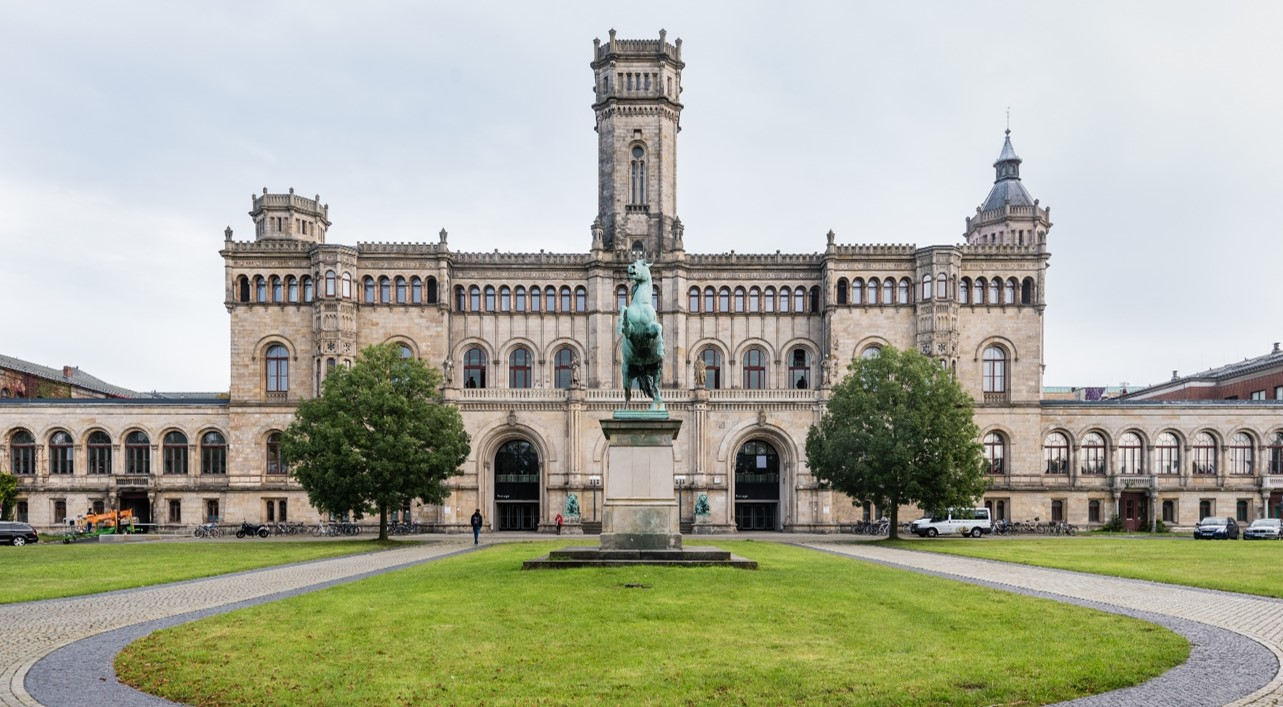
\includegraphics[width=0.65\textwidth]{figures/luh_default_presentation_title_image.jpg}}

% Title page: luhstyle
% \setbeamertemplate{title page}[luhstyle]
% % Add optional title image here
% \addtitlepageimage{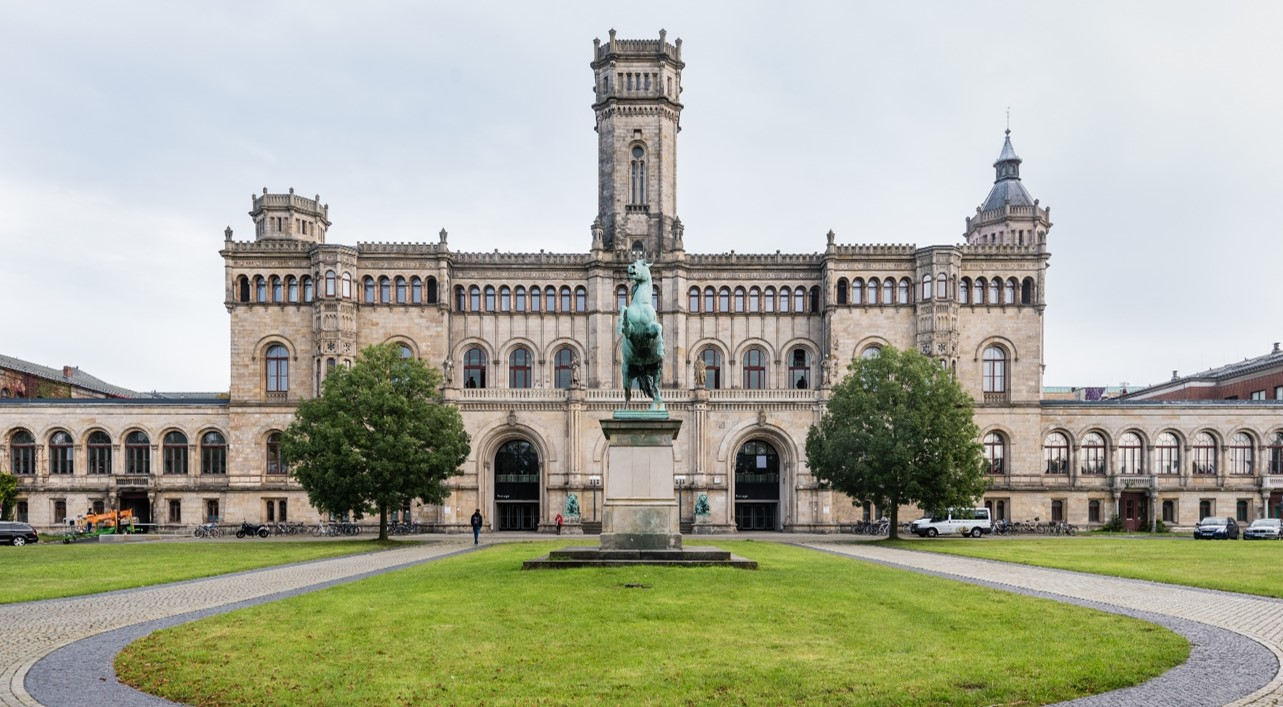
\includegraphics[width=0.75\textwidth]{figures/luh_default_presentation_title_image.jpg}}

\author[Abedjan \& Lindauer]{Ziawasch Abedjan \& Marius Lindauer\\[1em]
	
\includegraphics[height=\logoheight]{../latex_main/figures/luh_logo_rgb_0_80_155.pdf}\qquad
	
\includegraphics[height=\logoheight]{../latex_main/figures/DBIS_Kurzlogo.png}\qquad

\includegraphics[height=\logoheight]{../latex_main/figures/TNT_darkv4}\qquad

\includegraphics[height=\logoheight]{../latex_main/figures/L3S.jpg}	}
\date{Summer Term 2022; \hspace{0.5em} {
\includegraphics[height=1.5em]{../latex_main/figures/Cc-by-nc-sa_icon.svg.png}}; based on \href{https://ds100.org/fa21/}{[DS100]}
}


%%% Custom Packages
%----------------------------------------------------------------------
% Create dummy content
\usepackage{blindtext}

% Adds a frame with the current page layout. Just call \layout inside of a frame.
\usepackage{layout}


%%% Macros
%\renewcommand{\vec}[1]{\mathbf{#1}}
% \usepackage{bm}
%\let\vecb\bm

\title[Regression]{DS: Simple Linear Regression}
\subtitle{Model interpretation}

\graphicspath{ {./figure/} }
%\institute{}


\begin{document}
	
	\maketitle
	\begin{frame}{Interpreting slopes}
	    \begin{align*}
	        slope= r\frac{\sigma_y}{\sigma_x}
	    \end{align*}
	    The slope is measured in units of $y$ per unit of $x$.
	    \begin{itemize}
	        \item For instance, suppose we survey several individuals for their weight and height, and we want to use weight ($x$) to predict height ($y$). 
	        \begin{itemize}
	            \item Another way of saying this is “regressing height on weight.”
	        \end{itemize}
	        \item The units of our slope could be cm per kg.
	        \begin{itemize}
	            \item In a standard line $y = a + bx$, the slope ($b$) measures the increase in y for a 1 unit increase in x.
	        \end{itemize}
	    \end{itemize}
	    Using the above example, suppose our model turns out to be 
	    \begin{align*}
	           \text{predicted height = 56 + 0.09$\cdot$ weight}
	    \end{align*}
	\end{frame}
	
	
	\begin{frame}{Interpreting slopes}
	    \begin{align*}
	           \text{predicted height = 56 + 0.09$\cdot$ weight}
	    \end{align*}
	    Does this mean that if someone in the dataset puts on 1kg, we estimate that they will get $0.09$cm taller? No!
	    \begin{itemize}
	        \item The model we created shows association, not causation.
	        \item The data we collected is a snapshot of several people at one instance of time (cross-sectional), not snapshots of people over time (longitudinal).
	     \end{itemize}
	    What does this mean, then?

	    \begin{itemize}
	        \item $0.09$cm is the estimated height difference between two people whose weights are 1kg apart. 
	    \end{itemize}
	\end{frame}
	
	
	\begin{frame}{New data needs to be similar to original data}
	    \begin{columns}
    	    \begin{column}{.7\textwidth}
    	           Suppose we fit a model that predicts a Chihuahua’s weight given its length.
            	    \begin{align*}
            	           \text{predicted weight = 3 + 2$\cdot$length}
            	    \end{align*}
            	    Should we use this model to predict the weight of Great Danes? 
            	    \begin{itemize}
            	        \item No – we have no indication that the weight vs. length relationship for Great Danes are the same as Chihuahuas.
            	        \item Great Danes’ weights and lengths are well outside of the range of weights and lengths we fit our model on.
            	        \item If the new data we test our model on looks nothing like the data we fit our model on, there’s no guarantee that it will be any good.
            	        \begin{itemize}
            	            \item This is a notion we will formalize in a few lectures.
            	        \end{itemize}
            	     \end{itemize}
    	    \end{column}
	  
	        \begin{column}{.3\textwidth}
    	           \begin{figure}
    	               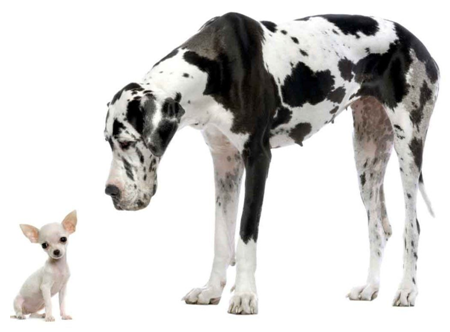
\includegraphics[scale=.3]{Bild7}
    	           \end{figure}
    	           Chihuahuas (left) range from 3-6 pounds, and 9.5-15 inches in length. Great Danes (right) range from 110-175 pounds, and 35.5-43 inches in length.
    	    \end{column}
	       \end{columns}
	\end{frame}
	
	
	\begin{frame}{Visualize, then quantify!}
	  
	    \begin{columns}
    	    \begin{column}{.6\textwidth}
    	           Anscombe’s quartet refers to the following four sets of points on the right.
            	    \begin{itemize}
            	        \item  They each have the same mean of $x$, mean of $y$, SD of $x$, SD of $y$, and $r$ value.
            	        \item Since our optimal SLR model only depends on those quantities, they all have the same regression line.
            	        \item However, the SLR model only makes sense as a model for one of these four sets of points.
            	        \item Before modeling, you should always visualize your data first!
            	     \end{itemize}
    	    \end{column}
	  
	        \begin{column}{.4\textwidth}
    	           \begin{figure}
    	               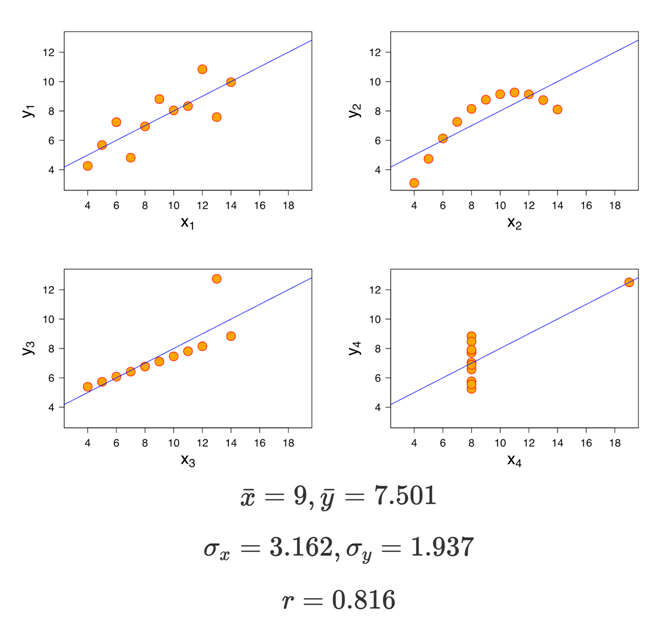
\includegraphics[scale=.33]{Bild8}
    	           \end{figure}
    	    \end{column}
	       \end{columns}
	\end{frame}
\end{document}